% I used overleaf

\documentclass[11pt]{amsbook}
\usepackage[turkish]{babel}
\usepackage{../Ceyhun}
\usepackage{../amsTurkish}
\usepackage{lipsum}

\begin{document}
% ++++++++++++++++++++++++++++++++++++++
\hPage{133}
% ++++++++++++++++++++++++++++++++++++++
birden çok dalını içerdiği için bu ağacın bir t-kesitlemesi değildir. Çizgede, $K_2$ yi t-kesitleme yapacak birçok ağacın bulunduğu gözden kaçmamalıdır. % Writer used "bir çok" but it is "birçok"

  \begin{figure}[htb]
  \centering
  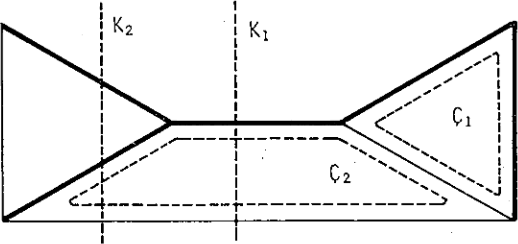
\includegraphics[width=0.6\textwidth]{images/ceyhun-133-fig01}
  \caption{Ağaç ve t-çevre ve t-kesitleme kavramlarının açıklanması.}
  \label{fig:3.2.1}
  \end{figure}
  
  \begin{theorem}
  A, \textbf{Ç} deki bir ağaç ve $a_i$ bu ağacın dalı olsun. $a_i$ nin tanımıayacağı t-kesitlemede, $a_i$ ile çevre yapan kirişler ve yalnız bu kirişler vardır. 
  \end{theorem}
  
\textit{Tanıt}

$a_i$ ayrıtının uç düğümlerini $A$ ve $B$ olarak simgeleyelim. Öyleyse $A$ daki düğümler, Şekil 3.2.2 de açıklandığı gibi $A$ türü ve $B$ türü diye iki kümeye ayrılabilir. Çizgedeki ayrıtlar da, yalnız

\end{document}